\documentclass[../main.tex]{subfiles}
\graphicspath{{\subfix{../../images/}}}

\begin{document}

Embedded systems are computers that serve \emph{just one purpose}, usually fitted within a device, like a lamp or toaster, to give it "smart" functionality.

They have the following components:

\begin{itemize}
    \item a \textbf{microprocessor}, which is a type of CPU (see section \ref{3:sec:cpu} for details) that serves as the central component of the embedded system. This may come in the form of:
        \begin{itemize}
            \item \textbf{a microcontroller}, which is a CPU with some RAM and ROM on a single chip. They can only carry out basic tasks and cannot load an operating system (see section \ref{4:sec:the_os_and_kernel}).
            \item \textbf{a microprocessor}, which is just a CPU without RAM or ROM. They must be added separately.
            \item \textbf{an SoC (System-on-a-Chip)}, which is a CPU, with RAM, ROM, and also chips that handle I/O (keyboards, mice, sensors, actuators), and secondary storage all in one package. They can mostly handle an OS.
        \end{itemize}
    \item \textbf{Input devices}, most often including sensors of some sort, to detect data in the surrounding environment. For example, a toaster might need a temperature sensor to see how hot the toast is. See section \ref{3:sec:input_and_output_devices} for details.
    \item \textbf{Output devices}, like a display, to show users information. In the case of a toaster, maybe a menu to display the types of toast it can cook, and how long before the toast is ejected. There may also be \textbf{Actuators}. See section \ref{3:sec:input_and_output_devices} for details.
\end{itemize}

\subsection{Event Loops}

This term is \emph{not necessarily in your syllabus}, but is the name for how these devices function.

Embedded systems typically runs instructions in a constant loop with the same structure, which is as follows:

\begin{enumerate}
    \item \textbf{Input polling:} Ask the input devices for any inputs.
    \item \textbf{Processing:} If the input devices gave the microprocessor some data, it processes it.
    \item \textbf{Output:} If the device needs to make an output, it is done at this stage.
\end{enumerate}

The following diagram better explains it:

\begin{figure}[H]
    \centering
    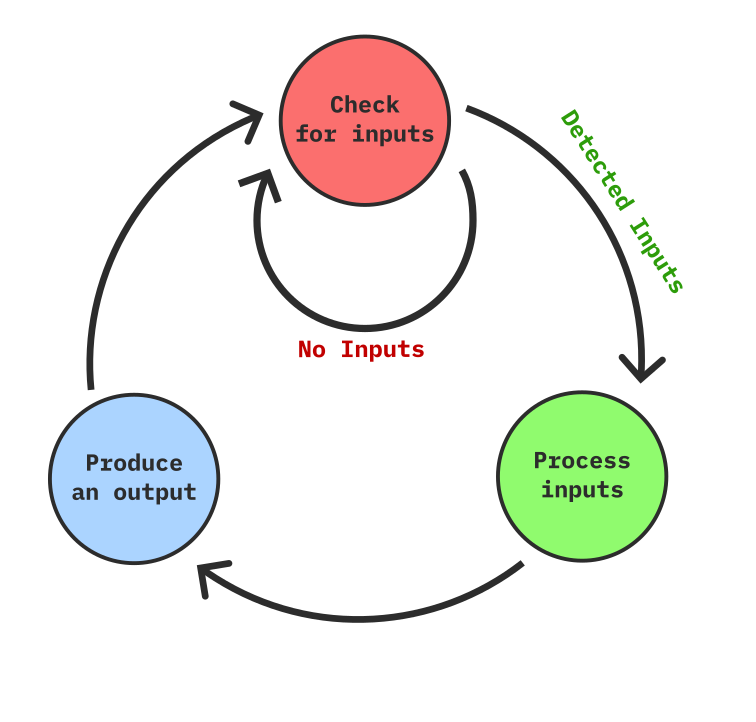
\includegraphics[width=0.7\textwidth]{eventloop.png}
    \caption{A typical event loop followed by embedded systems}
    \label{fig:eventloop}
\end{figure}

Some other notes include:

\begin{itemize}
    \item Data from sensors that provide \emph{analog data} will likely go through an ADC as a part of processing.
    \item All of this stuff is also called a \textbf{monitoring system}, which they will more likely use in the exam.
    \item For more case studies, check the relevant sections in the textbook.
\end{itemize}


\end{document}
